\item \textbf{{[}RVHS/PRELIM/9569/2021/P2/Q4{]} }

\textbf{Car Loaning System }

CaRent is a company providing electronic car rental services. The
company engages you to design a web application using Flask microframework
to aid in the car rental process. 

The following information of each Customer is stored: 

\texttt{CustomerID} -- auto increment integer value to keep track
of the ID of customer. 

\texttt{Name} -- name of customer. 

\texttt{Gender} -- gender of customer, to be stored as a single character,
using either '\texttt{M}' or '\texttt{F}'. 

\texttt{Contact} -- contact number of customer. 

The following information of each Car is stored: 

\texttt{VIN} -- vehicle identification number (VIN) of the car. 

\texttt{Brand} -- brand of the car. 

\texttt{Vehicle Type} -- type of the car, can be \texttt{'Sedan'},
\texttt{'Hatchback'}, \texttt{'SUV'} or \texttt{'MPV'}. 

\texttt{Energy Source} -- type of energy source the engine is running
on, can be \texttt{'Diesel'}, \texttt{'Gasoline'}, \texttt{'Hybrid'}
or \texttt{'Electricity'}. 

\texttt{DailyPrice} -- daily price for renting the car. 

\texttt{Availability} -- availability of the car, can be \texttt{'Available'}
or \texttt{'Unavailable'}. 

The following information of each RentalPoint is stored: 

\texttt{PointID} -- auto increment integer value to keep track of
the ID of rental service point.

\texttt{Address} -- address of the rental point. 

\texttt{OpWeekDay} -- weekdays that the rental point is open, stored
as a 7-digits string, starting from Sunday to Saturday, with \texttt{'1'}
indicating open and \texttt{'0'} indicating closed. E.g. \texttt{'0111110'}
means it is open on weekdays and closed on weekend. 

\texttt{OpStartHr} -- starting time of daily operation, stored as
a 4 digits string, using 24hour time format. 

\texttt{OpEndHr} -- ending time of daily operation, stored as a 4
digits string, using 24hour time format. 

The following information of each \texttt{RentalRecord} is stored: 

\texttt{CustomerID} -- ID of customer. 

\texttt{VIN} -- VIN of car. 

\texttt{StartDate} -- start date for the rental service. 

\texttt{CollectionPointID} -- ID of the collection point. 

\texttt{ReturnDate} -- return date for the rental service. 

\texttt{ReturnPointID} -- ID of the return point. 

The information is to be stored in four tables: 

\texttt{Customer} 

\texttt{Car} 

\texttt{RentalPoint} 

\texttt{RentalRecord} 

\subsubsection*{Task 4.1 }

Create an SQL file called \texttt{Task4\_1.sql} to show the SQL code
to create the database \texttt{car\_rental.db} with the three tables. 

The table \texttt{Customer} must use \texttt{CustomerID} as its primary
key, the table \texttt{Car} must use \texttt{VIN} as its primary key,
and the table \texttt{RentalPoint} must use \texttt{PointID} as its
primary key. 

The table \texttt{RentalRecord} should use \texttt{CustomerID}, \texttt{VIN}
and \texttt{StartDate} as a composite key, while \texttt{CustomerID},
\texttt{VIN} and \texttt{CollectionPointID/ReturnPointID} must refer
to \texttt{CustomerID} in \texttt{Customer}, \texttt{VIN} in \texttt{Car}
and \texttt{PointID} in \texttt{RentalPoint} as foreign keys. 

Save your SQL code as \texttt{Task4\_1.sql} \hfill{} {[}6{]}

\subsubsection*{Task 4.2 }

The files \texttt{customers.csv}, \texttt{cars.csv}, \texttt{rental\_points.csv}
and \texttt{rental\_records.csv} contains information about the customers,
cars, rental points and the past rental records. The first row of
each file contains the header of the respective columns. Each row
in the files is a comma- separated list of information. 

Write a Python program to insert all information from the three files
into the \texttt{database car\_rental.db}. Run the program. 

Save your program code as \texttt{Task4\_2.py} \hfill{}{[}6{]}

\subsubsection*{Task 4.3 }

You are tasked to implement a function to search and display all past
rental records of a customer. Using the customer\textquoteright s
name \texttt{\textbf{'Goh Yi Xi'}}, query and display a list of data
with the following fields as shown in the table, sorted in the ascending
order according to the start date. 
\noindent \begin{center}
\begin{tabular}{|c|c|c|c|c|c|}
\hline 
Name  & Contact  & VehicleType  & StartDate  & ReturnDate  & DailyPrice\tabularnewline
\hline 
\dots{}  & \dots{} & \dots{}  & \dots{}  & \dots{} & \dots{}\tabularnewline
\hline 
\end{tabular}
\par\end{center}

Write the SQL code required. 

Save this code as \texttt{Task4\_3.sql} \hfill{} {[}5{]}

\subsubsection*{Task 4.4 }

The company wants to implement a function to register new cars for
rental into the database. Office staff can register new cars by adding
the values of the attributes in the \texttt{Car} table. 

Write a Python program and the necessary files to create a web application
that: 
\begin{itemize}
\item Receive the following information: 
\begin{itemize}
\item \texttt{VIN}, \texttt{Brand}, \texttt{VehicleType}, \texttt{EnergySource},
and \texttt{DailyPrice} of a car through a HTML form.
\item \texttt{Availability} should be set to the default value of \texttt{'Available'}. 
\item Note that \texttt{VehicleType} and \texttt{EnergySource} should be
in \textbf{dropdown} list format to improve data validity. 
\end{itemize}
\item Check if the \texttt{VIN} is valid based on the following algorithm: 
\begin{itemize}
\item Step 1: Translate all letters to integer values using the following
table (\texttt{I}, \texttt{O}, and \texttt{Q} are not allowed in a
valid \texttt{VIN}): 
\noindent \begin{center}
\begin{tabular}{|c|c|c|c|c|c|c|c|c|}
\hline 
\textbf{A}: 1  & \textbf{B}: 2  & \textbf{C}: 3  & \textbf{D}: 4  & \textbf{E}: 5  & \textbf{F}: 6  & \textbf{G}: 7  & \textbf{H}: 8  & \textbf{N/A}\tabularnewline
\hline 
\textbf{J}: 1  & \textbf{K}: 2  & \textbf{L}: 3  & \textbf{M}: 4  & \textbf{N}: 5  & \textbf{N/A}  & \textbf{P}: 7  & \textbf{N/A } & \textbf{R}: 9\tabularnewline
\hline 
\textbf{N/A}  & \textbf{S}: 2  & \textbf{T}: 3  & \textbf{U}: 4  & \textbf{V}: 5  & \textbf{W}: 6  & \textbf{X}: 7  & \textbf{Y}: 8 & \textbf{Z}: 9\tabularnewline
\hline 
\end{tabular}
\par\end{center}
\item Step 2: Use the following weight factor for each position in the VIN.
\textbf{The 9th position is that of the check digit}. Its weight factor
has been substituted with a \texttt{0}, which will cancel it out in
the multiplication step. 
\noindent \begin{center}
\begin{tabular}{|c|c|c|c|c|c|c|c|c|c|c|c|c|c|c|c|c|c|}
\hline 
\textbf{Position } & \textbf{1 } & \textbf{2 } & \textbf{3} & \textbf{4} & \textbf{5} & \textbf{6} & \textbf{7} & \textbf{8} & \textbf{9} & \textbf{10} & \textbf{11} & \textbf{12} & \textbf{13} & \textbf{14} & \textbf{15} & \textbf{16} & \textbf{17}\tabularnewline
\hline 
Weight  & 8  & 7  & 6  & 5  & 4  & 3  & 2  & 10  & 0  & 9  & 8  & 7  & 6  & 5 & 4 & 3 & 2\tabularnewline
\hline 
\end{tabular}
\par\end{center}
\item The sum of product of the letter/digit with their corresponding weight
factor is then divided by \texttt{11}. 
\item The remainder is the check digit. If the remainder is \texttt{10},
the check digit will use \texttt{X} instead. 
\item E.g. the \texttt{VIN} with values 1\texttt{M8GDM9A\_KP042788} will
produce a check digit of \texttt{X} and hence \texttt{1M8GDM9AXKP042788}
is a valid \texttt{VIN}. 
\end{itemize}
\item If \texttt{VIN} is valid, create a new car record in the \texttt{Car}
table, and display the record in the confirmation page. 
\item Otherwise, inform the user that the VIN is invalid. 
\end{itemize}
\begin{center}
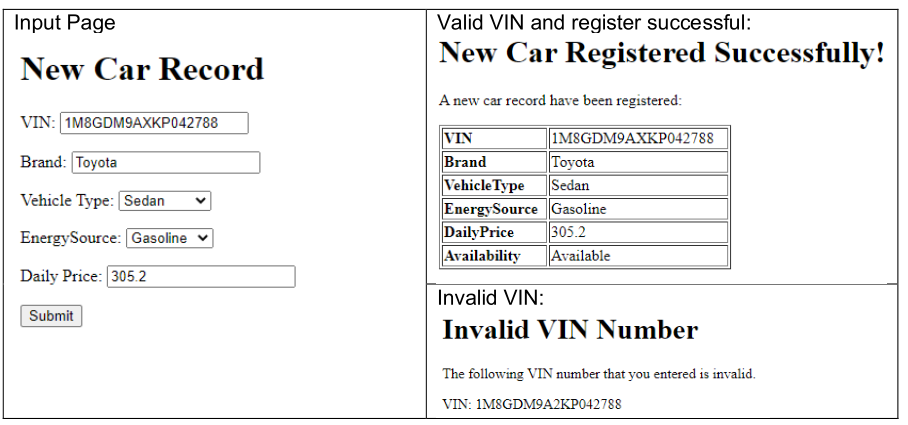
\includegraphics[width=0.5\paperwidth]{C:/Users/Admin/Desktop/Github/question_bank/LyX/static/img/9569-RVHS-2021-P2-Q4}
\par\end{center}

You may assume: 
\begin{itemize}
\item All inputs are in valid format. 
\item VIN: 1M8GDM9AXKP042788 is a new record to the database 
\end{itemize}
Save your program as \texttt{Task4\_4.py }

With additional files or sub-folders as needed in a folder named \texttt{Task4\_4 }

Run the web application. Enter the values based on the sample input
above. 

Then save the output of the program as \texttt{Task4\_4.html}. \hfill{}{[}15{]}